% Plantilla del artículo del Proyecto Integrador (Producto de difusión)
% Archivos necesarios en la misma carpeta: logo.jpeg, figura_ejemplo.png y referencias.bib
\documentclass[letterpaper,11pt]{article}

% --- Idioma y tipografía ---
\usepackage[T1]{fontenc}
\usepackage{lmodern}
\usepackage[spanish,es-tabla]{babel}

% --- Página: carta, márgenes 2.5 cm, interlineado 1.15 ---
\usepackage[margin=2.5cm]{geometry}
\geometry{headheight=52pt,headsep=0.3cm}
\usepackage{setspace}
\setstretch{1.15}

% --- Figuras y tablas ---
\usepackage{graphicx}
\usepackage{booktabs}
\usepackage{float}
\usepackage[font=small,labelfont=bf,labelsep=colon]{caption}

% --- Encabezado: logo (logo.jpeg) solo en la primera página ---
\usepackage{fancyhdr}
\renewcommand{\headrulewidth}{0pt}
\fancypagestyle{plain}{%
  \fancyhf{}%
  \fancyhead[C]{
\includegraphics[height=1.2cm]{logo.jpeg}}%
  \fancyfoot[C]{\thepage}}
\pagestyle{fancy}
\fancyhf{}
\fancyfoot[C]{\thepage}

% --- Cuadros de "Nota de formato" ---
\usepackage[skins,breakable]{tcolorbox}
\newtcolorbox{nota}{%
  enhanced, breakable,
  colback=black!8, colframe=black!8,
  boxrule=0pt, arc=0pt,
  left=3pt, right=3pt, top=2pt, bottom=2pt,
  before skip=10pt, after skip=10pt,
  fontupper=\sffamily\footnotesize\setstretch{1}
}

% --- Encabezados de sección ---
\usepackage{titlesec}
\titleformat{\section}{\Large\bfseries}{\thesection.}{0.6em}{}
\titleformat{\subsection}{\large\bfseries}{\thesubsection.}{0.6em}{}
\titlespacing*{\section}{0pt}{1.6ex plus 0.4ex minus 0.2ex}{1ex}

% --- Referencias: deje UNA de las dos líneas activa ---
\usepackage{csquotes}
\usepackage[style=apa,backend=biber]{biblatex}      % APA 7
% \usepackage[style=ieee,backend=biber]{biblatex}   % IEEE
\addbibresource{referencias.bib}

% --- Enlaces y URL (DOI); se carga al final ---
\usepackage[hidelinks]{hyperref}
\urlstyle{same}

% --- Título ---
\title{\textbf{Título del proyecto}}
\author{Integrante 1\quad Integrante 2\\[2pt] Integrante 3\\[6pt]
  \normalsize Proyecto Integrador · Maestría en Inteligencia Artificial Aplicada \\[6pt]
  \normalsize Asesor: Nombre del asesor \quad·\quad Fecha de entrega}
\date{\vspace{-2ex}}

\begin{document}

\maketitle

% --- Resumen (sin número) ---
\begin{abstract}
El resumen ocupa un solo párrafo de 150 a 250 palabras. Se escribe al final, cuando las cifras del artículo ya están cerradas, y debe entenderse sin leer el resto: qué problema se atendió, con qué datos, qué se obtuvo y qué se recomienda. Este párrafo es solo un ejemplo de su ubicación y de su forma.
\end{abstract}

\begin{nota}
\textbf{Nota de formato.} Las ocho partes van en este orden: Resumen; Contexto de negocio y problema; Datos y preparación; Metodología y modelos; Resultados y validación; Implementación y operación; Conclusiones clave; Referencias y anexos. El resumen y las referencias no llevan número; las demás secciones y sus subsecciones, sí. Este ejemplo muestra solo dos secciones.
\end{nota}

% --- Sección 1 ---
\section{Contexto de negocio y problema}
Las citas siguen un solo estilo en todo el artículo. En APA~7 se cita con autor y año, ya sea dentro de la oración, como \textcite{breiman2001}, o entre paréntesis al final de una idea \parencite{hastie2009}. Cuando se usa una biblioteca de software conviene citarla también \parencite{pedregosa2011}.

% --- Sección 4 (el ejemplo salta a la numeración 4) ---
\setcounter{section}{3}
\section{Resultados y validación}
Toda figura y toda tabla se menciona en el texto antes de aparecer: la
Figura~\ref{fig:ejemplo} muestra una serie ilustrativa y la Tabla~\ref{tab:ejemplo}, un resumen con intervalos.

\begin{nota}
\textbf{Nota de formato.} Figuras y tablas numeradas, con pie; el pie de la figura va debajo y el de la tabla, arriba. Las cifras del artículo coinciden con las de los cuadernos ya entregados. Tablas extensas (por ejemplo: búsquedas de hiperparámetros) van a los anexos y el cuerpo las resume.
\end{nota}

% --- Figura 1 (pie debajo) ---
\begin{figure}[H]
  \centering
  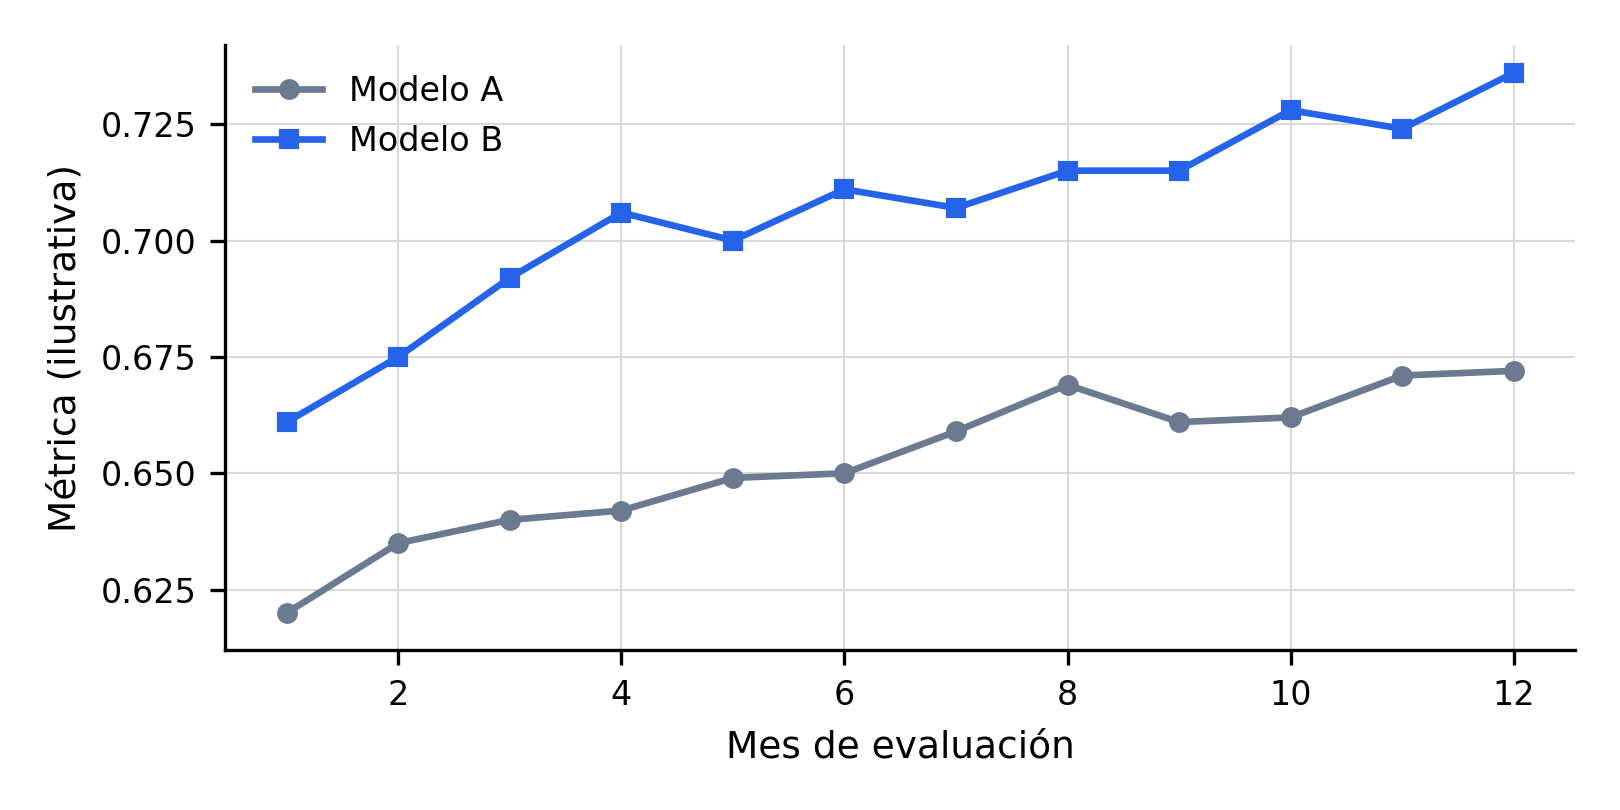
\includegraphics[width=0.82\linewidth]{figura_ejemplo.png}
  \caption{Pie de figura: dice qué se muestra y cómo leerlo (ejes, unidades, qué comparar). Datos ilustrativos.}
  \label{fig:ejemplo}
\end{figure}

% --- Tabla 1 (pie arriba) ---
\begin{table}[H]
  \centering
  \caption{Pie de tabla, arriba de la tabla: qué contiene y de dónde salen las cifras. Valores ilustrativos.}
  \label{tab:ejemplo}
  \begin{tabular}{lcr}
    \toprule
    Modelo & Métrica & Intervalo de 95\,\% \\
    \midrule
    Referencia & 0.62 & [0.60, 0.64] \\
    Modelo A   & 0.66 & [0.64, 0.68] \\
    Modelo B   & 0.71 & [0.69, 0.73] \\
    \bottomrule
  \end{tabular}
\end{table}

% --- Declaración de uso de IA (antes de las referencias) ---
\section*{Declaración de uso de inteligencia artificial}
Se utilizó \textcite{anthropic2026claude} para \textcolor{red}{[indicar la finalidad]}.
La responsabilidad final sobre el contenido entregado recae en los autores.

% --- Referencias (biblatex + Biber, solo lo citado) ---
\printbibliography[title={Referencias}]

% --- Anexos (en página nueva; \appendix cambia la numeración a A, B, ...) ---
\clearpage
\appendix
\section{Título del anexo}
Los anexos se titulan y se citan desde el cuerpo (por ejemplo, «véase el Anexo~A»).

\end{document}
